\documentclass{article}
\title{Funktionale Programmierung Mitschrieb}
\usepackage{fancyhdr}
\pagestyle{fancy}
\usepackage{hyperref}
\usepackage{enumerate}
\usepackage{amsmath}
\usepackage{amsfonts}
\usepackage{amssymb}
\usepackage{nicefrac}
\fancyhf{}
\fancyhead[C]{Torsten Grust - Functional Programming}
\usepackage{fontspec}
\setmonofont{Andale Mono}
\usepackage[english]{babel}
\author{Finn Ickler}
\usepackage{mdframed}
\usepackage{tikz}
\usepackage{epigraph}
\usepackage{minted}
\renewcommand{\listingscaption}{Code example}
\newcommand{\Haskell}[1]{\mintinline{Haskell}{#1}}
\setcounter{secnumdepth}{-1}
\hypersetup{%
pdfborder = {0 0 0}
}
\begin{document}
\maketitle
\epigraph{\glqq Avoid success at all cost \grqq}{Simon Peyton Jones}
\tableofcontents
\listoflistings
\section{Vorlesung 1}
\begin{listing}
\caption{Hello World}
\begin{minted}{haskell}
-- Hello World Haskell
main :: IO ()
main = putStrLn "Chewie, we're home"
\end{minted}
\end{listing}
\subsection{Functional Programming (FP)}
A programming language is a medium for expressive ideas (not to get a computer to perform operations ). Thus programs must be written for people to read, and only incidentally for machines.
\subsection{Computational Model in FP : \emph{Reduction}}
Replace expressions by their value.\\
IN FP, expressions are formed by applying functions to values.
\begin{enumerate}
\item Function as in maths: $x = y \rightarrow f(x) = f(y)$
\item Functions are values like numbers or text
\end{enumerate}
\begin{tabular}{l|c|c}
&FP&Imperative\\
construction & function application and composition & statement sequencing\\
execution & reduction (expression evaluation) & state changes\\
semantics & $\lambda$-calculus&denotational
\end{tabular}\bigskip\\
$ n \in \mathbb{N}, n \geq 2$ is a prime number $\Leftrightarrow$ the set of non-trivial factors of n is empty.\\
$n$ is prime $\Leftrightarrow \{ m \mid m \in m \in \{2,\ldots,n-1\}, n mod m = 0 \} = \{\}$\\
\begin{listing}[h!]
\begin{minted}{c}
int IsPrime(int n)
{
    int m;
    int found_factor;
    found_factor
    for (m = 2; m <= n -1; m++)
    {
        if (n % m == 0)
        {
            found_factor = 1 ;
            break;
        }
    }
    return !found_factor;
}
\end{minted}
\caption{isPrime in C}
\end{listing}
\begin{listing}[h!]
\begin{minted}{Haskell}
isPrime :: Integer -> Bool
isPrime n = factors n == []
  where 
    factors :: Integer -> [Integer]
    factors n = [ m  | m <- [2..n-1], mod n m == 0]

main :: IO ()
main = do
  let n = 42
  print (isPrime n)
\end{minted}
\caption{isPrime in Haskell}
\end{listing}
\newpage
\usemintedstyle[Haskell]{bw}
\definecolor{bg}{rgb}{0.95,0.95,0.95}
\begin{listing}[h!]
\begin{minted}[bgcolor=bg]{Haskell}
let xs = [ x+1 | x <- [0..9] ]
:sprint xs = _
length xs
:sprint xs = [_,_,_,_,_,_,_,_,_]
\end{minted}
\caption{Lazy Evaluation in der ghci REPL}
\end{listing}
\usemintedstyle[Haskell]{default}
\subsection{Haskell Ramp Up}
Read $\equiv$ as ''denotes the same value as''\\
Apply f to value e:\quad f \textvisiblespace e \\(juxtaposition, ''apply'', binary operator \textvisiblespace, Haskell speak: infixL 10 \textvisiblespace)
= \textvisiblespace has max precedence (10): f $e_1$ +$e_2 \equiv $(f $e_1$) + $e_2$
\textvisiblespace associates to the left g \textvisiblespace f \textvisiblespace e $\equiv$ (g f) e
Function composition:
\begin{enumerate}[-]
\item g (f e)
\item Operator ''.'' (''after'') : (g.f) e (. = $\circ$) = g(f (e))
\item Alternative ''apply'' operator \$ (lowest precedence, associates to the right), infix 0\$): f\$$e_1$+ $e_2$ = f ($e_1 + e_2$)
\end{enumerate}
\section{Vorlesung 2}
\begin{listing}
\caption{Verschiedene Schreibweise einer Applikation}
\begin{minted}[bgcolor=bg]{Haskell}
cos 2 * pi
cos (2 * pi)
cos $ 2 * pi
isLetter (head (reverse ("It's a " ++ "Trap")))
(isLetter . head . reverse ) ("It's a" ++ "Trap")
isLetter $ head $ reverse $ "It's a" ++ "Trap"
\end{minted}
\end{listing}
\noindent Prefix application of binary infix operator $\oplus$
\begin{minted}[escapeinside=||]{Haskell}
(|$\oplus) e_1 e_2 \equiv e_1 \oplus e_2$|
|$(\&\&)$| True False |$\equiv$| False
\end{minted}
Infix application of binary function f:
\begin{minted}[escapeinside=||]{Haskell}
|$e_1$| `f` |$e_2$| |$\equiv$| f |$e_1 e_2$|
x `elem` xs |$\equiv$| x |$\in$| xs
\end{minted}
User defined operators with characters : \mintinline{Haskell}|!#%&*+/<=>?@\^|~|
\begin{listing}
\caption{Eigener $\approx$ Opperator}
\begin{minted}{Haskell}
epsilon :: Double
epsilon = 0.00001
(~=~) :: Double -> Double -> Bool
x ~=~ y = abs (x - y) < epsilon
infix 4 ~=~ 
\end{minted}
\end{listing}
\subsection{Values and Types}
Read \mintinline{Haskell}|::| as ''has type''\\
Any Haskell value e has a type t (\mintinline{Haskell}{e::t}) that is determined at compile time.\\
The \mintinline{Haskell}|::| type assignment is either given explicitly or inferred by the computer
\subsection{Types}
\begin{tabular}{lll}
Type&Description&Value\\
\hline
Int & fixed precision integers ($-2^{63}\ldots2^{63}-1$)&\Haskell{0,1,42}\\
Integer & arbitrary Precision integers & \Haskell{0,10^100}\\
Float,Double & Single/Double precision floating points & \Haskell{0.1,1e03}\\
Char & Unicode Character&\mintinline[escapeinside=||]{Haskell}{'x','\t', '△', '\8710'}\\
Bool & Booleans & \mintinline[escapeinside=||]{Haskell}{True, False}\\
() & Unit (single-value type) & \mintinline[escapeinside=||]{Haskell}{()}
\end{tabular}
\begin{minted}[bgcolor =bg]{Haskell}
2
it :: Integer
42 :: Int 
it :: Int
'a' 
it :: Char
True 
it :: Bool
10^100 
it :: Integer
10^100 :: Double 
it :: Double
\end{minted}
\subsection{Type Constructors}
\begin{itemize}
\item Build new types from existing Types
\item Let a,b denote arbitrary Types (type variables)
\end{itemize}
\begin{tabular}{lp{6cm}l}
Type Constructor& Description & Values\\
\hline
(a,b)&pairs of values of types a and b& \Haskell{(1,True) :: (Int, Bool)}\\
($\text{a}_1,\text{a}_2,\ldots,\text{a}_n$)& n-Types& \Haskell{2,False :: (Int, Bool)}\\
\Haskell{[a]} &list of values of type a & \Haskell{[] :: [a]}\\
\Haskell{Maybe} a & optional value of type a & \Haskell{Just 42 Maybe Integer}\\
& & \Haskell{Nothing :: Maybe a}\\
\Haskell{Either} a b & Choice between values of Type a and b& \Haskell{Left 'x' :: Either Char b}\\
& & \Haskell{Right pi :: Either a Double}\\
\Haskell{IO} a & I/O action that returns a value of type a (can habe side effects ) & \Haskell{print 42 :: IO} ()\\
& & \Haskell{getChar :: IO Char}\\
a \Haskell{->} b & function from type a to b & \Haskell{isLetter :: Char -> Bool}
\end{tabular}
\begin{minted}[bgcolor=bg]{Haskell}
(1, '1', 1.0)
it :: (Integer, Char, Double)
[1, '1', 1.0]
it :: Fehler
[0.1,1.0,0.01] 
it :: [Double]
[]
it :: [t]
"Yoda"
it :: [Char]
['Y', 'o', 'd', 'a']
"Yoda"
[Just 0, Nothing, Just 2] 
it :: [Maybe Integer]
[Left True, Right 'a']
it :: [Either Bool Char]
print 'x' 
it :: ()
getChar
*
it :: Char
:t getChar
getChar :: Io Char
:t fst 
fst :: (a,b) -> a
:t snd
snd :: (a,b) -> b
:t head
head :: [a] -> a
:t (++)
(++) :: [a] -> [a] -> [a]
\end{minted}
\subsection{Currying}
\begin{itemize}
\item Recall:\begin{enumerate}
\item $e_1$ \Haskell{++} $e_2 \equiv$ \Haskell{(++)} $e_1 e_2$
\item \Haskell{++} $e_1 e_2 \equiv$ \Haskell{((++)} $e_1) e_2$
\end{enumerate}
\item Function application happens one argument at a time (currying, Haskell B. Curry)
\item Type of n-ary function: : $a_1$ \Haskell{->} $a_2$ \Haskell{... ->} $a_n$ \Haskell{-> b}
\item Type constructor \Haskell{->} associates to the right thus read the type as:\\ $a_1$ \Haskell{->} ($a_2$ \Haskell{->} $a_3$ (\Haskell{... ->} ($a_n$ \Haskell{-> b})\ldots))
\item Enables partial application: ''Give me a value of type $a_1$, I'll give you a (n-1)-ary function of type $a_2$ \Haskell{->} $a_3$ \Haskell{-> ... ->} $a_n$ \Haskell{-> b}
\end{itemize}
\begin{minted}[bgcolor = bg]{Haskell}
"Chew" ++ "bacca"
"Chewbacca"
(++) "Chew" "bacca"
"Chewbacca"
((++) "Chew") "bacca"
"Chewbacca"
:t (++) "Chew"
"Chew" :: [Char] -> [Char]
let chew = (++) "Chew"
chew "bacca"
"Chewbacca"
let double (*) 2
double 21
42
\end{minted}
\section{Vorlesung 3}
\subsection{Defining Values (and thus: Functions)}
\begin{itemize}
\item = binds names to values, names must not start with A-Z (Haskell style: camelCase)
\item Define constant (0-ary) c, value of c is that of expression:\\
c = e
\item Define n-ary function, arguments $x_i$ and f may occur in e (no "letrec" needed)\\
f $x_1\ x_2\ldots x_n = e$
\item Hskell programm = set of top-level bindings (order immaterial, no rebinding)
\item Good style: give type assignment for top-level bindings:\\
\Haskell{f :: a1 -> a2 -> b}\\
\Haskell{f } $x_1$ $x_2$ \Haskell{= e}
\begin{listing}[h!]
\caption{fac in Haskell}
\begin{minted}{Haskell}
fac :: Integer -> Integer
fac n = if n <= 1 then 1 else n * fac (n - 1)

fac2 n | n <= 1    = 1
       | otherwise = n * fac2 (n - 1)

main :: IO ()
main = print $ fac 10
\end{minted}
\end{listing}
\item Guards (introduced by $\vert$).
\begin{minted}[escapeinside=@@]{Haskell}
f @$x_1\ x_2\ \ldots\ x_n$@
  |@$q_1$@ = @$e_1$@
  |@$q_2$@ = @$e_n$@
\end{minted}
\begin{listing}[h!]
\caption{Power in Haskell}
\begin{minted}{Haskell}
power :: Double -> Integer -> Double
power x k | k == 1 = x
          | even k = power (x * x) (halve k)
          | otherwise = x * power (x * x) (halve k)
  where
    even :: Integer -> Bool -- Nicht typisch
    even n  = n `mod` 2 == 0
    halve n = n `div` 2

main :: IO ()
main = print $ power 2 16 
\end{minted}
\end{listing}
\item $q_i$ (expressions of type Bool) evaluated top to bottom, first True guards ''wins''\\
$\mathrm{fac}\ n = \begin{cases}
1 &if n \geq 1\\
n \cdot \mathrm{fac(n-1)}& else
\end{cases}$\\
\end{itemize}
\subsection{Lokale Definitionen}
\begin{enumerate}
\item \Haskell{where} - binding : Local definitions visible in the entire right-hand-side (rhs) of a definition
\begin{minted}[escapeinside=@@]{Haskell}
f @$x_1\ x_2\ \ldots\ x_n$@
  |@$q_1$@ = @$e_1$@
  |@$q_2$@ = @$e_n$@
 where 
    @$g_1$@ ... = @$b_1$@
    @$g_i$@ ... = @$b_i$@
\end{minted}
\item \Haskell{let} - expression Local definitions visible inside an expression:
\begin{minted}[escapeinside=@@]{Haskell}
let @$g_1$@ ... = @$b_1$@
    @$g_2$@ ... = @$b_1$@
in e
\end{minted}
\end{enumerate}
\section*{Haskells 2-dimensionale Syntax (Layout) (Forumbeitrag)}
\begin{mdframed}
Hallo zusammen,\\
in der dritten Vorlesung hatte ich erwähnt, dass Haskells Syntax darauf verzichtet, Blöcke (von Definitionen) mittels Sonderzeichen abzugrenzen und zu strukturieren. 
Andere Programmiersprachen bedienen sich hier typischerweise Zeichen wie {, } und ;.\\
Haskell baut hingegen auf das sog. Layout, eine Art 2-dimensionaler Syntax.  Wer schon einmal Python und seine Konventionen zur Einrückung von Blöcken hinter for und if kennengelernt hat, wird hier Parallelen sehen. 
Die Regelungen zu Layout lauten wie folgt und werden vom Haskell-Compiler während der Parsing-Phase angewandt:
\begin{itemize}
\item The first token \textbf{after} a \Haskell{where/let} and the \textbf{first token of a top-level definition} define the upper-left corner of a box.
\item The first token left of the box closes the box (offside rule).
\item Insert a \textit{\{} before the box.
\item Insert a \textit{\}} after the box.
\item Insert a \textit{;} before each line that starts at left box border.
\end{itemize}
Die Anwendung dieser Regeln auf dieses Beispielprogramm:
\begin{minted}{Haskell}
let y   = a * b       
    f x = (x + y) / y 
in  f c + f d
\end{minted}

führt zur Identifikation der folgenden Box:
\begin{verbatim}
   ┌──────────┄┄     
let│y   = a * b      
   │f x = (x + y) / y
   └──────────┄┄     
\end{verbatim}
\Haskell{in  f c + f d}\\  
Das Token in in der letzten Zeile steht links von der Boxgrenze im Abseits (siehe die offside rule).  Der Parser führt nun die Zeichen {, } und ; ein und verarbeitet das Programm so, als ob der Programmierer diese Zeichen explizit angegeben hätte.  (Haskell kann alternativ übrigens auch in dieser sog. expliziten Syntax geschrieben werden — das ist aber sehr unüblich, hat negativen Einfluss aufs Karma und ist vor allem für den Einsatz in automatischen Programmgeneratoren gedacht.)\\
Die explizite Form des obigen Programmes lautet (nach den drei letzten Regeln):
\begin{minted}{Haskell}
let {y   = a * b       
    ;f x = (x + y) / y}
in  f c + f d 
\end{minted}     
Damit ist die Bedeutung des Programmes eindeutig und es ist klar, dass bspw. nicht das folgende gemeint war (in dieser alternativen Lesart ist das Token f aus der zweiten in die erste Zeile "gerutscht"):
\begin{minted}{Haskell}
let y = a * b f    
    x = (x + y) / y
in  f c + f d   
\end{minted}
Aus diesen Layout-Regeln ergeben sich recht einfache Richtlinien für das Einrücken in Haskell-Programmen:
\begin{itemize}
\item Die Zeilen einer Definition auf dem Top-Level beginnen jeweils ganz links (Spalte 1) im Quelltext.
\item Lokale where / let-Definitionen werden um mindestens ein Whitespace (typisch: 2 oder 4 Spaces oder 1 Tab) eingerückt.
\item Es gibt in Haskell ein weiteres Keyword (do, wird später thematisiert), das den gleichen Regeln wie where / let folgt.
\end{itemize}
Beste Grüße,\\
\phantom{ }\qquad —Torsten Grust
\end{mdframed}
\subsection{Lists([a])}
\begin{itemize}
\item Recursive definition:
\begin{enumerate}
\item\Haskell{[]} ist a list (nil), type \Haskell{[] :: [a]}
\item\Haskell{x : xs} (head, tail) is a list, if \Haskell{x :: a}, and \Haskell{xs :: [a]}.\\
\phantom{ }\quad \Haskell{cons: (:) :: a -> [a] -> [a] -> [a]} with \Haskell{infixr : 5}
\end{enumerate}
\item Notation: \Haskell{3:(2:1:[])} $\equiv$ \Haskell{3:2:1:[]} $\equiv$ \Haskell{[3,2,1]}
\end{itemize}
\begin{minted}[bgcolor =bg]{Haskell}
[]
it :: [t]
[1]
it :: [Integer]
[1,2,3]
it :: [Integer]
['z']
"z"
it :: [Char]
['z','x']
"zx"
it :: [Char]
[] == ""
True
it :: Bool
[[1],[2,3]]
it :: [[Integer]]
[[1],[2,3],[]]
[[1],[2,3]]
it :: [[Integer]]
False:[]
[False]
it :: [Bool]
(False:[]):[]
it ::[[Bool]]
:t [(<),(<=),(>)]
[(<),(<=),(>)] :: Ord a => [a -> a-> Bool]
[(1,"one"),(2,"two"),(3,"three")]
it :: [(Integer,[Char])]
:t head
head :: [a] -> a
:t tail :: [a] -> [a]
head "It's a trap"
'I'
it :: Char
tail  "It's a trap"
"t's a trap"
it :: [Char]
reverse "Never odd or even"
"neve ro ddo reveN"
it :: [Char]
\end{minted}
\begin{itemize}
\item Law
$\forall $\texttt{xs}$ \ne$\Haskell{[]}: \Haskell{head xs : tail} = \texttt{xs}
\end{itemize}
\begin{minted}[bgcolor =bg]{Haskell}
:i String
type String = [Char]
\end{minted}
\subsection{Type Synonyms}
\begin{itemize}
\item Introduce your own type synonyms. (type names : {\em U}ppercase)
\Haskell{type} $t_1$ \Haskell{=} $t_2$
\end{itemize}
\begin{minted}{Haskell}
type Bits = [Integer]

type Predicate a = a -> Bool

bits :: Integer -> Bits
bits n | n == 0    =[0]
       | otherwise = (n `mod` 2) : bits (n `div`2)

isEven :: Predicate Integer
isEven n = head (bits n) == 0

main :: IO ()
main = print $ isEven 35
\end{minted}
Sequence (lists of enumerable elements)
\begin{itemize}
\item \Haskell{[x..y]} $\equiv$ \Haskell{[x,x+1,x+2,...,y]}

\begin{minted}[bgcolor= bg]{Haskell}
['a'..'z']
"abcdefghijklmnopqrstuvwxyz"
\end{minted}
\item \Haskell{x,s..y}$\equiv$ \Haskell{[x,x+i,x+(2*i),...,y] where i = x-s}

\begin{minted}[bgcolor= bg]{Haskell}
[1,3..20]
[1,3,5,7,9,11,13,15,17,19]
[2,4..20]
[2,4,6,8,10,12,14,16,18,20]
\end{minted}
\item Infinite List \Haskell{[1..]}
\end{itemize}
\section{Vorlesung 4}
\subsection{Pattern Matching}
\emph{The} idiomatic way to define functions by cases:
\Haskell{f :: }$a_1$ \Haskell{->}$\ldots$\Haskell{->}$a_k$ \Haskell{-> b}\\
\Haskell{f} $p_{11} \ldots p_{1k} = e_1\\$
$\vdots\quad \vdots\quad \vdots\quad \vdots $\\
\Haskell{f} $p_{m1} \ldots p_{nk} = e_n$\\
For all $e_i$ \Haskell{:: b}
on $a_i$ call \Haskell{f} $x_1x_2\ldots x_k$ each $x_i$ is matched against patterns $p_{i1}\ldots p_{in}$ in order. Result is $e_r$ if the rth branch is the first in which all patterns match.\\
\begin{tabular}{lp{4cm}p{4cm}}
Pattern&Matches if\ldots&Bindings in $e_r$\\\hline
constant c&$x_1$ == c\\
variable v&always& v = $x_i$\\
wildcard \_ &always\\
tuple ($p_1,\ldots,p_n$)&components of $x_i$ match type component patterns& Those bound by the component patterns\\
$[]$& $x_i == []$\\
$p_1:p_2$&\Haskell{head} $x_1$ matches $p_1$, \Haskell{tail} $x_i$ matches $p_2$\\
$v@p$& p matches&those bound by $p$ and $v=x_i$
\end{tabular}\\
Note: In a pattern, a variable may only occur once (linear patterns only)
\begin{listing}
\caption{sum in Haskell}
\begin{minted}{Haskell}
--(1) if then else
sum' :: [Integer] -> Integer
sum' xs =
   if xs == [] then 0 else head xs + sum' (tail xs)
--(2) guards
sum'' :: [Integer] -> Integer
sum'' xs | xs == [] = 0
         | otherwise = head xs + sum'' (tail xs)
--(3) pattern matching
sum''' :: [Integer] -> Integer
sum''' []     = 0
sum''' (x:xs) = x + sum''' xs

main :: IO ()
main = do
  print $ sum' [1,2,3]
  print $ sum'' [1,2,3]
  print $ sum''' [1,2,3]
\end{minted}
\end{listing}
\begin{listing}\label{ageof.hs}
\caption{ageOf in Haskell}
\inputminted{Haskell}{ageOf.hs}
\end{listing}
\begin{listing}
\caption{take in Haskell}
\inputminted{Haskell}{take.hs}
\end{listing}
\begin{listing}
\caption{merge in Haskell}
\inputminted[]{Haskell}{merges.hs}
\end{listing}
\begin{listing}
\caption{mergeSort in Haskell}
\inputminted{Haskell}{mergesort.hs}
\end{listing}
\subsection{Pattern matching in expressions (case)}
\begin{minted}[escapeinside=@@]{Haskell}
case e of @$p_1$@ | @$q_{11}$@ -> @$e_{11}$@
          @$\vdots$@
          @$p_n$@ | @$q_{n1}$@ -> @$e_{n1}$@
\end{minted}
\clearpage
\section{Vorlesung 5}
\subsection{Algebraic Data Types (Sum of Product Types)}
\begin{itemize}
\item Recall: \Haskell{[]} and \Haskell{(:)} are the \emph{constructors} for Type \Haskell{[a]}
\item Can define entirely new Type T and its constructors $K_i$:
\subitem \begin{tabbing}
\Haskell{data T} $a_1\ a_2\ \ldots\ a_n $\=$ = K_1\ b{11}\ \ldots\ b_{1n_1}$\\
\>\  $| K_2\ b_{21}\ \ldots\ b_{2n_2}$\\
\>\  $\vdots\qquad \vdots$\\
\>\  $| K_r\ b_{r1}\ \ldots\ b_{rnr}$
\end{tabbing}
\item Defines \emph{Type constructor} T and r \emph{value constructor} with types
\item $\text{\Haskell{K}}_i$\Haskell{::}$b_{i1}\ldots\ b_{ini}$\Haskell{-> T}$a_1\ a_2\ldots\ a_n$
\item $K_i$ identifier with uppercase first letter or symbol starting with \Haskell{:}
\item Example: [weekday.hs]
\subitem - Sum (or enumeration, choice)
\end{itemize}
\begin{listing}[h!]
\caption{weekday.hs}
\inputminted{Haskell}{weekday.hs}
\end{listing}
\begin{minted}[bgcolor = bg]{Haskell}
Wed
No instance for (Show Weekday) arising from a use of print
Thu == Sun 
No instance for (Eq Weekday) arising from a use of '=='
Mon > Sat
No instance for (Ord Weekday) arising form a use of '>'
\end{minted}
\begin{itemize}
\item Add deriving \Haskell{(c,c,...,c)} to data declaration to define canonical (intuitive) operations:\\
\begin{tabular}{l|l}
c (class)&operations\\ \hline
\Haskell{Eq}&equality (\Haskell{==,/=})\\
\Haskell{Show}&printing (\Haskell{show})\\
\Haskell{Ord}&ordering  (\Haskell{<,<=,max})\\
\Haskell{Enum}&enumeration (\Haskell{[x..y]})\\
\Haskell{Bounded}& bounds (\Haskell{minBound,maxBound})
\end{tabular}
\end{itemize}
\begin{listing}[h!]
\caption{RockPaperScissors.hs}
\inputminted{Haskell}{RockPaperScissor.hs}
\end{listing}
\begin{listing}[h!]\label{sequence.hs}
\caption{sequence.hs}
\inputminted{Haskell}{sequence.hs}
\end{listing}
\begin{itemize}
\item Product, r = 1, $n_1 = 2$ (\ref{sequence.hs})
\item Sum of Products:
\subitem \Haskell{Maybe a} = \Haskell{Nothing | Just a}
\subitem \Haskell{data Either a b} = \Haskell{Left a | Right a}
\subitem \Haskell{List a = Nil} 
\subitem \phantom{List a}\ | \Haskell{Cons a (List a)}
\end{itemize}
\begin{listing}[h!]
\caption{cons.hs}
\inputminted{Haskell}{cons.hs}
\end{listing}
\begin{listing}[h!]
\caption{eval-compile-run.hs}
\inputminted{Haskell}{eval-compile-run.hs}
\end{listing}
\clearpage
\section{Vorlesung 6}
\subsection{Type Classes}
A Type class C defines a family of type signatures (''methods'') whichi all \emph{instances} of c must implement:\\
\begin{minted}[escapeinside=||]{Haskell}
class C where
|$f_1$| :: |$t_1$|
|$f_2$| :: |$t_2$|
   |$\vdots$|
|$f_n$| :: |$t_n$|
\end{minted}
The  $t_i$ \emph{must} mention a For any $f_i$, the class may provide default definitions (that instances may overwrite).\\
\begin{itemize}
\item Example
\begin{minted}{Haskell}
class Eq a where 
(==) :: a -> a -> Bool
(/=) :: a -> a -> Bool
x /= y = not (x == y)
x == y = not (x /= y)
\end{minted}
\end{itemize}
\subsection{Class Constraints}
A \emph{class constraint} \Haskell{e (a => :: t} (where t mentions a) says that e has type t \emph{only if} a is an instance of class C.\\
\begin{minted}[bgcolor=bg]{Haskell}
:t (+)
(+) :: Num a => a -> a -> a
:t print
print :: Show a => a -> IO ()
:hoogle +Data.List
Data.List sort :: Ord a => [a] -> [a]
:hoogle [(a,b)] -> a -> Maybe b
lookup :: Eq a => a -> a [(a,b)] -> Maybe b
\end{minted}
\begin{listing}[h!]
\inputminted{Haskell}{type-classes.hs}
\caption{Default implementation of Show, Ord and Enum}
\end{listing}
\subsection{Class inheritance}
Defining class $(c_1a,c_2a,\ldots)$ \Haskell{=>} (\Haskell{a where ...}) makes type class C a \emph{subclass} of the $c_1$ C inherits all methods of the $c_i$.\\
(\Haskell{a => t} implies $(c_1a,c_2a,\ldots,Ca)$\Haskell{=> t})
\clearpage
\includegraphics[scale=0.7]{classes.png}
\newpage
\subsection{Class Instances}
If type t implements the method of class C, t becomes an \emph{instance} of c:
\begin{minted}[escapeinside=||]{Haskell}
instance C t where
|$f_1$| = <def of |$f_1$|> --all f may be
       |$\vdots$|        --provided, minimal
|$f_n$| = <def of |$f_n$|> --complete definition
                --must be provided
\end{minted}
$\bullet$ Example:\\
\begin{minted}{Haskell}
instance Eq Bool where
  x == y = (x && y) || (not x && not y)

instance (Eq a, Eq b) => Eq (a,b) where
  (x1,y1) == (x2,y2) = x1 == x2 && y1 == y2

instance Eq a => Eq [a] where
  [] == []         = True
  (x:xs) == (y:ys) = x == y && xs == ys
  _      == _      = False

\end{minted}
$\bullet$ An instance definition for type constructor t may formulate type constraints for its argument types: a, b ... :\\
\Haskell{instance} ($c_1a,c_2,c_3b,\ldots)$ \Haskell{=>} 
 \Haskell{(t a b) where}\\
\begin{minted}[bgcolor=bg]{Haskell}
:i Enum
class Enum a where
  succ :: a -> a
  pred :: a -> a
  toEnum :: Int -> a
  fromEnum :: a -> Int
  enumFrom :: a -> [a]
  enumFromThen :: a -> a -> [a]
  enumFromTo :: a -> a -> [a]
  enumFromThenTo :: a -> a -> a -> [a]
  	-- Defined in ‘GHC.Enum’
instance Enum Word -- Defined in ‘GHC.Enum’
instance Enum Ordering -- Defined in ‘GHC.Enum’
instance Enum Integer -- Defined in ‘GHC.Enum’
instance Enum Int -- Defined in ‘GHC.Enum’
instance Enum Char -- Defined in ‘GHC.Enum’
instance Enum Bool -- Defined in ‘GHC.Enum’
instance Enum () -- Defined in ‘GHC.Enum’
instance Enum Float -- Defined in ‘GHC.Float’
instance Enum Double -- Defined in ‘GHC.Float’
fromEnum 'A'
65
fromEnum 'B'
66
toEnum 65
Exception: Prelude.Enum.().toEnum: bad argument
:t toEnum 65
toEnum 65 :: Enum a => a
toEnum 65 :: Char
'A'
toEnum 0 :: Bool
False
toEnum 20 :: Double
20.0
\end{minted}
\begin{listing}
\caption{Rock paper Scissors with instances}
\inputminted{Haskell}{RockPaperScissor-inheritance.hs}
\end{listing}
\subsection{Deriving Class Instances}
\begin{itemize}
\item Automatically made user-defined data (data ...) intsances of classes $c_i \in \{\text{\Haskell{Eq, Ord, Enum,Bounded, Show, Read}}\}$
\begin{minted}[escapeinside=@@]{Haskell}
data T @$a_1$@ @$a_2$@ ... @$a_n$@ = ...
                       |
  deriving (@$c_1$@..,@$c_n$@)
\end{minted}
\end{itemize}
\inputminted{Haskell}{RockPaperScissor-deriving.hs}
\clearpage
\section{Vorlesung 7}
\subsection{Domain Specific Languages}
\begin{itemize}
\item ''small languages'' designed to easily and directly express the concepts/idioms of a given domain. \emph{Not} Turing-complete in general. 
\item Examples:\qquad
\begin{tabular}{l|l}
	Domain         & DSL               \\ \hline
	Os automation  & Shell scripts     \\
	Typesetting    & \TeX, \LaTeX      \\
	Queries        & SQL               \\
	Game Scripting & UnrealScript, Lua \\
	Parsing        & Bison, ANTLR
\end{tabular}
\item Functional Languages are good hosts for Embedded DSLs:
\subitem- algebraic data types (e.g model abstract syntax trees)
\subitem- higher-order functions (e.g control constructs)
\subitem- lightweight syntax (layout/whitespace, non-alphabetic identifiers)
\end{itemize}
Example: An embedded DSL for finite sets of integers:\\
\begin{minipage}{.85\textwidth}
\begin{minted}{Haskell}
type IntegerSet = ...
empty  :: IntegerSet
insert :: Integer    -> IntegerSet -> IntegerSet
delete :: Integer    -> IntegerSet -> IntegerSet
member :: Integer    -> IntegerSet -> Bool
\end{minted}
\end{minipage}%
\begin{minipage}{.15\textwidth}
$\Biggl\} $construct.\\ \ \\
$\}$ observer
\end{minipage}\\
\Haskell{member 3 (insert 1 (delete 3 (insert 2 (insert 3 empty))))} $\rightarrow$ \Haskell{False}\\
DSL: \textcircled{1} Library of functions, implementaion details exposed
\begin{listing}[h!]
\caption{library-exposed.hs}
\inputminted{Haskell}{library-exposed.hs}
\end{listing}
\subsection{Modules}
Group related definitions (names, types) in a single file (named \verb|M.hs|)
\begin{minted}{Haskell}
module M where
type Predicate a = a -> Bool
id :: a -> a
id = \x -> x
\end{minted}
Hierarchy : module A.B.C.M in file \verb|A/B/C/M.hs|
\begin{itemize}
\item definitions in other module M:\\
\subitem \Haskell{import M}
\item Explicit export Lists hode all other definitions
\subitem \Haskell{module M (id) where ...}
\subsubitem \Haskell{--type Predicate a not exported} 
\item Abstract data types: export algebraic datatypes, but \emph{not} its constructor functions
\subitem \Haskell{module M (Rose, leaf) where}
\subitem \Haskell{data Rose a = Node a [Rose a] --constructor Node not exported}
\subitem \Haskell{leaf :: a -> Rose a}
\subitem \Haskell{leaf x = Node x []}
\item Export constructors:
\subitem \Haskell{module M (Rose (Node), leaf) where ...}
\subitem \Haskell{module M (Rose (...), leaf)  where ...}
\item Qualified imports to partition space:
\subitem \Haskell{import qualified M [as Nickname]}
\subitem \Haskell{t :: M.Rose Char}
\subitem \Haskell{t = M.leaf 'x'}
\end{itemize}
\begin{minted}[bgcolor =bg]{Haskell}
:t fromJust
Not in scope: ‘fromJust’
import Data.Maybe
:t fromJust
fromJust :: Maybe a -> a

import qualified Data.Maybe
:t Data.Maybe.fromJust
Data.Maybe.fromJust :: Maybe a -> a

import qualified Data.Maybe as DM
:t DM.fromJust
DM.fromJust :: Maybe a -> a
\end{minted}
\begin{itemize}
\item Partially import module:
\subitem \Haskell{import Data.List (nub,maybe)}
\subitem \Haskell{import Prelude hiding (otherwise)}
\subitem \Haskell{otherwise :: Bool}
\subitem \Haskell{otherwise = False}
\end{itemize}
\begin{listing}[h!]
\caption{Two implementations of the SetLanguage module}
\inputminted{Haskell}{SetLanguage.hs}
\inputminted{Haskell}{SetlanguageFunction.hs}
\end{listing}
\clearpage
\section{Vorlesung 8}
\begin{itemize}
\item Shallow DSL embedding : Semantiics of DSL operations directly expressed in terms of a host language value (e.g list or characteristic function).
\subitem- constructors (\Haskell{empty,insert,delete}) perform the work, harder to add
\subitem- Observer (\Haskell{member}) trivial
\item \emph{Deep} DSL embedding: DSL operations build an abstract syntax Tree (AST) that represents applications and arguments
\subitem- constructors merely build the AST, very easy to add
\subitem- observer: interpret (traverse) the AST and perform the work
\end{itemize}
\begin{listing}[h!]
\caption{SetLanguageDeep.hs}
\inputminted{Haskell}{SetLanguageDeep.hs}
\end{listing}
\begin{minted}[bgcolor=bg]{Haskell}
:i Num
class Num a where
  (+) :: a -> a -> a
  (-) :: a -> a -> a
  (*) :: a -> a -> a
  negate :: a -> a
  abs :: a -> a
  signum :: a -> a
  fromInteger :: Integer -> a
  	-- Defined in ‘GHC.Num’
instance Num Word -- Defined in ‘GHC.Num’
instance Num Integer -- Defined in ‘GHC.Num’
instance Num Int -- Defined in ‘GHC.Num’
instance Num Float -- Defined in ‘GHC.Float’
instance Num Double -- Defined in ‘GHC.Float’
:t 42
42 :: Num a => a
default ()
42
<interactive>:5:1:
    No instance for (Num a0) arising from a use of ‘it’
    The type variable ‘a0’ is ambiguous
    Note: there are several potential instances:
      instance Integral a => Num (GHC.Real.Ratio a)
        -- Defined in ‘GHC.Real’
      instance Num Integer -- Defined in ‘GHC.Num’
      instance Num Double -- Defined in ‘GHC.Float’
      ...plus three others
    In the first argument of ‘print’, namely ‘it’
    In a stmt of an interactive GHCi command: print it
default (Integer,Rational, Double)
42
42
42 / 3
14 % 1
42.1
421 % 10
default (Integer,Double)
\end{minted}
\begin{listing}[h!]
\caption{ExprDeepNum.hs}
\inputminted{Haskell}{ExprDeepNum.hs}
\end{listing}
\begin{listing}[h!]
\caption{ExprDeepNum.hs}
\inputminted{Haskell}{ExprDeep.hs}
\end{listing}
\clearpage
\subsection{Generalized Algebraic Datatypes}
Idea :
\begin{itemize}
\item Encode the type of a DSL expression (here : Integer or Bool) in its \emph{Haskell type}
\item Use Haskell's type checker to ensure at \emph{compile time} that only well-typed DSL expressions are built:
\end{itemize}
\subsection{GADTs}
\begin{itemize}
\item Language extensions: \Haskell{{-# LANGUAGE GADTs #-}}
\item Define entirely new parameters \Haskell{Type T}, its (value) constructors $k_i$ and their type signatures
\begin{minted}[escapeinside=||]{Haskell}
data T |$a_1\ a_2\ \ldots\ a_n$| where
  |$k_1$| :: |$b_{11}$| -> ... |$b_{1n_1}$| -> T |$t_{11}\ t_{12} \ldots\ t_{1n}$|
  |$k_2$| :: |$b_{21}$| -> ... |$b_{2n_2}$| -> T |$t_{21}\ t_{22} \ldots\ t_{2n}$|
...
\end{minted}
\end{itemize}
\begin{listing}[h!]
\caption{ExprDeepTyped.hs}
\inputminted{Haskell}{ExprDeepTyped.hs}
\end{listing}
\clearpage
\section{Vorlesung 9}
\begin{listing}[h!]
\caption{ExprEmbedding.hs}
\inputminted{Haskell}{ExprEmbedding.hs}
\end{listing}
\begin{listing}
\caption{expr-embeddings.hs}
\inputminted{Haskell}{expr-embeddings.hs}
\end{listing}
\subsection{Shallow Embedding of a String Matching DSL}
\begin{itemize}
\item Pattern:
\begin{enumerate}[1.]
\item Given a string, a pattern returns a \emph{list of matches.} Match failure?\marginpar{Replace failure by a list of successes} return the \emph{empty list} (of matches)
\item A match consists of a value (e.g the match of characters, tokens parse tree) and the residual string to match\\
Thus: \Haskell{type Pattern a = String -> [(a,String)]}
\epigraph{A pattern of things is list of things and strings}{Torsten Grust, 10.12.2015}
\end{enumerate} 
\item DSL design:\\
\begin{tabular}{l|l}
Pattern& DSL Function \Haskell{Char -> String ([Char,String])}\\ \hline
match literal& \Haskell{lit :: Char -> Pattern Char}\\
match empty string& \Haskell{empty :: a -> Pattern a}\\
fail always & \Haskell{fail :: Pattern a}\\
alternative &\Haskell{alt :: Pattern a -> Pattern a -> Pattern a}\\
sequence &\Haskell{seq ::(a ->  b -> c)-> Pattern a -> Pattern b -> Pattern c}\\
repetition & \Haskell{Pattern a -> Pattern [a]}
\end{tabular}
\end{itemize}
\begin{listing}
\inputminted{Haskell}{PatternMatching.hs}
\end{listing}
\begin{listing}
\inputminted{Haskell}{pattern-match.hs}
\end{listing}
\clearpage
\section{Vorlesung 10}
\subsection{Lazy Evaluation}
To execute a programm, Haskell \emph{reduces} expression to values. Haskell uses \emph{normal order reduction} to select the next expression to reduce:
\begin{itemize}
\item The \emph{outermost} reducable expression (redex) is reduced first.
\item $\Rightarrow$ Function application are reduced first \emph{before} their arguments.
\item If no further redex is found, the expression is in \emph{normal form}. and reduction terminates.
\end{itemize}
\begin{minted}[escapeinside=||]{Haskell}
fst :: (a,b) -> a
fst (x,y) = x
sqr :: Num a => a -> a
sqr x = x * x
---------------
fst (sqr (1 + 3), sqr 2) |$\rightarrow$| sqr (1 + 3)        [fst]
                         |$\rightarrow$| (1 + 3) * (1 + 3)  [sqr]
                         |$\rightarrow$| 4 * 4              [+/+]
                         |$\rightarrow$| 16                 [*]
\end{minted}
\begin{minted}{racket}
(define-racket-procedures pair
  make-pair
  pair?
  (pair-fst)
  (pair-snd))

(define fst
  (lambda (p)
    (pair-fst p)))

(define sqr 
  (lambda (x) (* x x)))

;Racket uses applicative order reduction (innermost first)
\end{minted}
\begin{listing}[h!]
\caption{This Programm compiles in Haskell, but not in Racket}
\inputminted[]{Haskell}{bomb.hs}
\end{listing}
Haskell avoids the duplication of work through \emph{graph reduction}: Expression are shared (referenced more than once) instead of duplicated. Reduction of \Haskell{sqr (1 + 3)}:\\
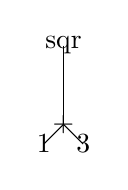
\begin{tikzpicture}
\node at (0,0) {sqr};
\draw (0,0) -- (0,-1);
\node at (0,-1) {+};
\draw (0,-1) -- (0.25,-1.25);
\node at (0.25,-1.25) {3};
\draw (0,-1) -- (-0.25,-1.25);
\node at (-0.25,-1.25) {1};
\end{tikzpicture}$\rightarrow$
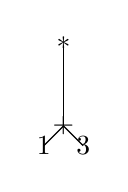
\begin{tikzpicture}
\node at (0,0) {*};
\draw (0,0) -- (0,-1);
\node at (0,-1) {+};
\draw (0,-1) -- (0.25,-1.25);
\node at (0.25,-1.25) {3};
\draw (0,-1) -- (-0.25,-1.25);
\node at (-0.25,-1.25) {1};
\end{tikzpicture}\\
Lazy evaluation: normal order reduction + sharing + WHNF\\
\emph{thunks}
\subsection{WHNF}
An expression $e$ ist in \emph{weak head normal form} (WHNF) if it is of the following form:\\
\newcommand{\iu}[1]{\textcircled{\raisebox{-0.1em}{#1}}}
\begin{enumerate}[\iu{1}]
\item \Haskell{v} (where \Haskell{v} is an \emph{atomic} value \Haskell{Integer, Char, Bool,...})
\item[\iu{2}] $c\ e_1\ e_2\ \ldots e_n$ (where $c$ is an n-ary constructor (like \Haskell{(:)} ))
\item[\iu{3}] $f\ e_1\ e_2 \ \ldots e_m$ (where f is a n-ary function, $m < n$)
\end{enumerate}
Haskell reduces values to WHNF only (stop criteria for reducion) unless we request reduction to normal fprm (e.g when printing result)\\
\subsection{Example expressions in WHNF}
\begin{minted}[escapeinside=||]{Haskell}
42 -- |\iu{1}|
(sqr 2,sqr 4) -- |\iu{2}|
f x = map f xs -- |\iu{2}| (:)
Just (40 + 2) -- |\iu{2}| Just
(* (40 + 2)) --  |\iu{3}| * binary
(\x -> 40 + 2) --  |\iu{3}| * binary
\end{minted}
\begin{minted}[bgcolor=bg]{Haskell}
(1 + 3) : []
[4]
it :: [Integer]
let xs = (1 + 3) : []
xs :: [Integer]
:sprint xs 
xs = [_]
\end{minted}
\subsection{Lazy Evaluation and Bottom ($\perp$)}
Some Haskell expressions have the value \emph{bottom} ($perp$) Examples: \Haskell{error ".."}, \Haskell{undefined}, \Haskell{bomb}. Lazy evaluation admits functions that return a non-bottom value even if they receive $\perp$ as an argument (also:{\em non-Strict functions }).
N-ary function is \emph{strict} in its i-th argument, if $f\ x_1\ \ldots\ x_{i-1} \perp x_{i+1} \ldots x_n = \perp$\\
Examples:
\begin{itemize}
\item \Haskell{const :: a -> b -> a} strict in first, non-strict in second argument
\item \Haskell{(&&) :: Bool -> Bool -> Bool}
\end{itemize}
$\bigtriangleup\! \hspace*{-0.45em}!\hspace*{0.45em}$ If a function \emph{pattern matches} an argument, Haskell semantics define it to be strict in that argument.\\
Example:\\
\begin{minted}[escapeinside=||]{Haskell}
data T = T Int
f :: T -> Int
f (T x) = 42
f undefined     |$\rightarrow$| undefined
f (T undefined) |$\rightarrow$| 42
\end{minted}
\begin{listing}[h!]
\inputminted{Haskell}{bottom.hs}
\caption{Bottom type}
\end{listing}
\begin{listing}[h!]
\inputminted{Haskell}{min.hs}
\caption{Finding the minimum by sorting the list}
\end{listing}
\begin{minted}[escapeinside=||]{Haskell}
min [8,6,1,7,5] |$\rightarrow$| (head . isort (<)) [8,6,1,7,5]  [min]
|$\rightarrow$| head (isort (<) [8,6,1,7,5])                    [(.)]
|$\rightarrow$| head (ins 8 (ins 6 (ins 1 (ins 7 (ins 5 []))))) [isort.2*]
|$\rightarrow$| head (ins 8 (ins 6 (ins 1(ins 7 [8]))))         [ins.1]
|$\rightarrow$| head (ins 8 (ins 6 (ins 1 (5 : ins 7 []))))     [ins.3]
|$\rightarrow$| head (ins 8 (1 : ins 6 ( 5 : ins 7 [])))        [ins.2]
|$\rightarrow$| (1 : ins 8 (ins 6 (5 : ins 7 [])))              [ins.3]
|$\rightarrow$| 1
\end{minted}
\begin{minted}[bgcolor=bg]{Haskell}
min [1..1000000]
1
it :: Integer
(1.50 secs, 521,738,256 bytes)
min [1..10000000]
1
it :: Integer
(15.43 secs, 5,164,721,896 bytes)
\end{minted}
\clearpage
\section{Vorlesung 11}
\subsection{Infinite Lists (Data Structures)}
One consequence of lazy evaluation, programs can handle \emph{infinite Lists} as long as any run will inspect onlt a finite prefix of such a list.\\
Enables a modular programming style:\\
\begin{enumerate}
\item \textbf{generator functions} produce an infinite number of solutions/approximations
\item \textbf{test functions} select one (or finite number of) solutions from this infinie list)
\end{enumerate}
Example: Newton-Raphson square root approximation
Iteratively approximate the square root of $x$
\begin{enumerate}
\item $a_0 = \nicefrac{x}{2}$
\item $a_{i+1} = \nicefrac{(a_i + \nicefrac{x}{a_i})}{2}$\hfill$a = (a + \nicefrac{x}{a}/2) \Leftrightarrow a = \sqrt{x}$
\end{enumerate}
\inputminted{Haskell}{sqrt.hs}
Example (Tic-Tac-Toe game tree):\\
Build the (potentially huge) \emph{tree of possible moevs} for the Tic-Tac-Toe Board game. Evaluate promise of game position.\\
Plan:\\
\begin{enumerate}
\item[\textcircled{1}] Find representation of game position (board + player next up)\\
\begin{tabular}{|l|l|l|}
\hline
1&2&3 \\ \hline
4&5&6 \\ \hline
X&O&X \\ \hline
\end{tabular}
\item[\textcircled{2}]provide pretty-printing for game
\item[\textcircled{3}]Define initial position and possible moves : \Haskell{moves :: Position -> [Position]}
\item[\textcircled{4}] Evaluate a given position: \Haskell{static :: Position -> Int}
\end{enumerate}
\inputminted{Haskell}{tic-tac-toe.hs}
\end{document}